\documentclass[tikz,border=4pt]{standalone}
\usepackage{graphicx}
\usepackage{xcolor}

\definecolor{goliatblue}{RGB}{65,91,105}

\begin{document}
\begin{tikzpicture}[font=\rmfamily\small]
  \node[font=\rmfamily\bfseries] at (4.15,6.62) {Worker Monitoring};
  \node[inner sep=0pt, draw=black, line width=0.6pt, anchor=south west] at (0,0)
    {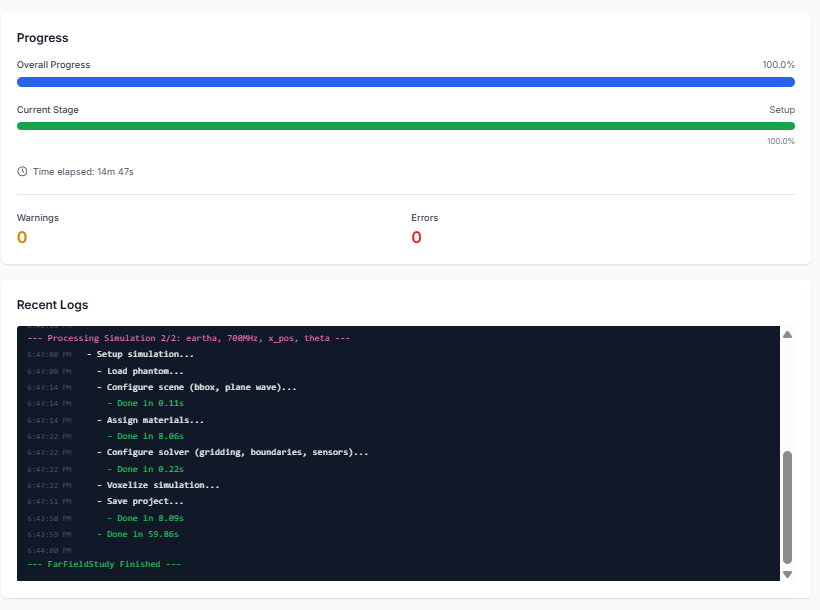
\includegraphics[width=8.30cm]{monitoring_worker_crop.png}};

  \node[font=\rmfamily\bfseries] at (12.75,6.62) {Extracted Point Field};
  \node[inner sep=0pt, draw=black, line width=0.6pt, anchor=south west] at (8.60,0)
    {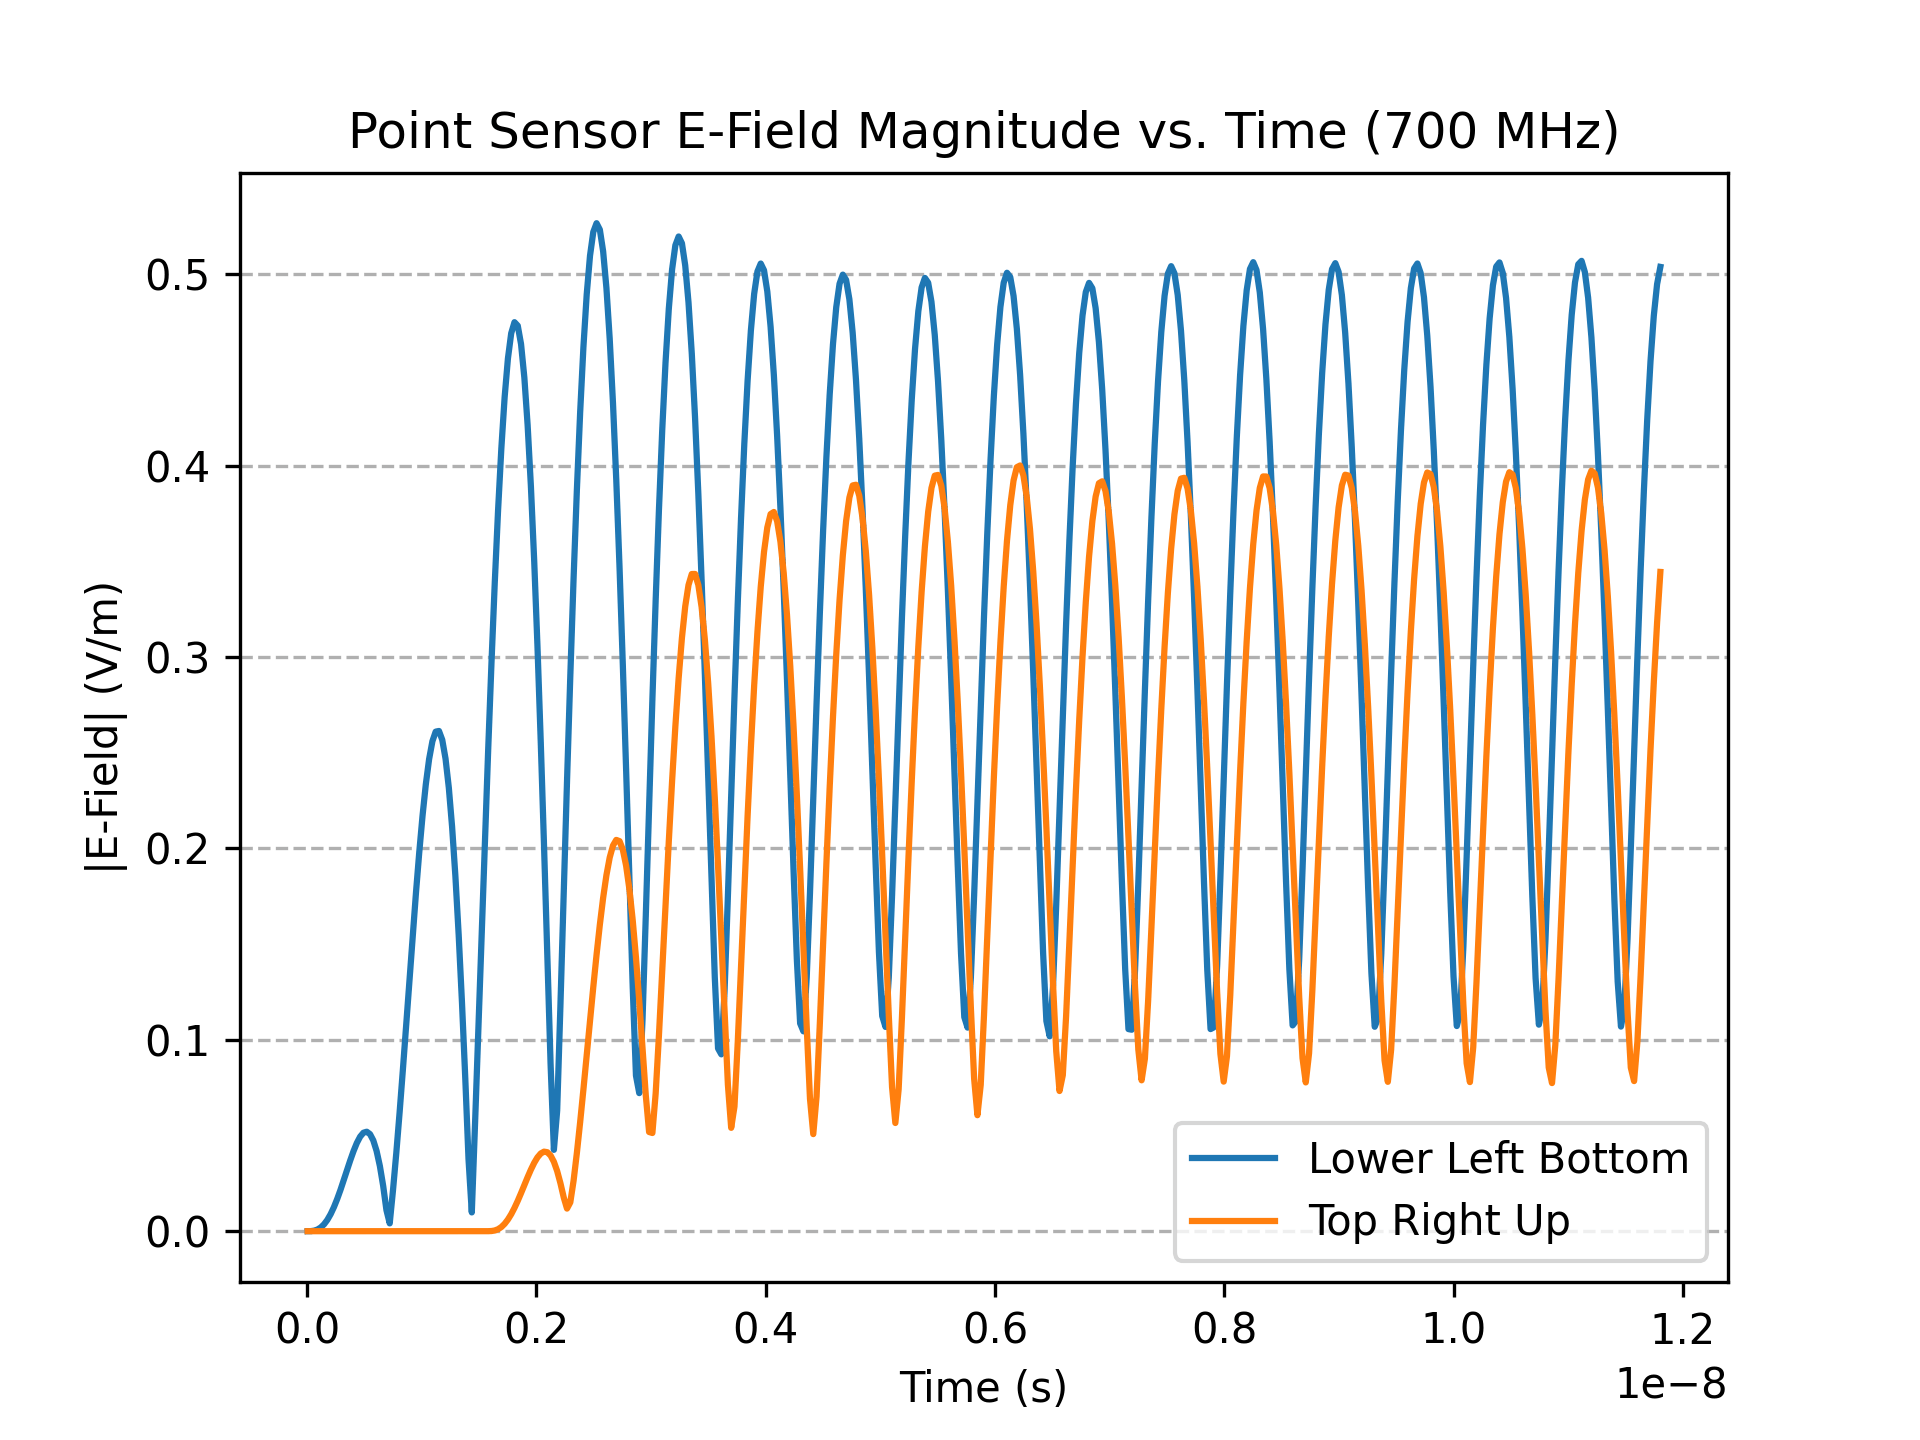
\includegraphics[width=8.30cm]{point_sensor_plot.png}};
\end{tikzpicture}
\end{document}
